
\documentclass{llncs}
\usepackage[tbtags]{amsmath}
\usepackage{amsfonts}
\usepackage{algorithm,algorithmic}
\usepackage{mathtools}
\usepackage{graphicx}
\usepackage{subfig}
\usepackage{tabu}
\DeclarePairedDelimiter\abs{\lvert}{\rvert}
\DeclarePairedDelimiter\norm{\lVert}{\rVert}

\def \y {\mathbf{y}}
\def \x {\mathbf{x}}
\def \Y {\mathbf{Y}}
\def \X {\mathbf{X}}
\def \w {\mathbf{w}}
\def \W {\mathbf{W}}
\def \v {\mathbf{v}}
\def \V {\mathbf{V}}
\def \Z {\mathbf{Z}}
\def \z {\mathbf{z}}
\def \b {\mathbf{b}}
\def \s {\mathbf{s}}

\renewcommand{\algorithmicrequire}{\textbf{Input:}}
\renewcommand{\algorithmicensure}{\textbf{Output:}}


%
\begin{document}
	\title{Learning the local coding scheme: Jointly Optimized Locally Linear Classifiers }
	\author{Teng Zhang \inst{1} \and Chenghao Liu \inst{1} \and Peilin Zhao \inst{2} \and Steven C.H. Hoi \inst{3} \and Jianling Sun \inst{1}}
	\institute{School of Computer Science and Technology, Zhejiang University, China
	\and
	Artificial intelligence department, Ant Financial, China
	\and
	School of Information Systems, Singapore Management University, Singapore
	\\
	\email{faramita@zju.edu.cn, twinsken@zju.edu.cn, peilin.zpl@antfin.com, chhoi@smu.edu.sg, sunjl@zju.edu.cn}}	
	\maketitle
	
	\begin{abstract}
		 Kernel Support Vector Machine (Kernel SVM) has been widely used in classification task due to their capability of training nonlinear data. However, the high computational cost of Kernel SVM prevents it from processing large scale datasets. To address this problem, locally linear classifiers have been proposed to approximate the nonlinear decision boundaries with a predefined local coding scheme. The power of locally linear classifiers depends heavily on the quantity of anchor points chosen and local codes. Existing methods usually employ a predefined local coding and unsupervised anchor points learning, followed by supervised classifier training, which is sub-optimal as the classification task is not exploited in discovering more suitable local coding scheme and anchor points,  and thus can result in a sub-optimal local codes and anchor points for classification task. In this paper, we propose a unified framework that learns the local codes, anchor points and model parameters in a jointly optimization problem. Our jointly optimized locally linear classifiers model can be effectively learned in an online fashion by stochastic gradient decent method. Experimental results on real-world datasets validate the effectiveness of our proposed methods. 
 	\end{abstract}
	
	\section{Introduction}
	Support Vector Machine (SVMs) are widely used in classification task. Although kernel tricks \cite{1} enables SVM to perform well in nonlinear dataset, the high computational cost still prevents kernel SVM from being used on many large datasets. To tackle this issue, locally linear classifiers \cite{2} \cite{3} have been proposed to approximate nonlinear decision boundaries using a predefined local coding scheme. The key point is to locally embed each data point into a lower dimension space, expressed as coordinates with respect to a set of surrounding anchor points.
	
	Typically, for locally linear classifiers based on local coding method, three vital ingradients need to be carefully defined. Firstly, the quality of anchor points chosen has a significant impact on the model's performance. Most of the locally linear classifiers initialize the anchor points in an unsupervised fashion \cite{2} \cite{5}. To refine the anchor points learning phase, a novel framework is discussed \cite{4} in which anchor points along with classifiers is learned jointly by a fully supervised approach. Secondly, choose the surrounding anchor points in local coding scheme. To avoid a high computational cost and hurting the classfication performance due to the ignorance of underlying local manifold structure, most locally linear classifiers \cite{2} \cite{4} take KNN algorithm \cite{7} to select $k$-nearest anchor points for following local coding step for each data point. The value of $k$ is fixed for each dataset and usually chosen via cross-validation, which is a kind of naive and exhausting method. Thirdly, the local coding scheme should be predefined. In other words, a rule of soft-assignment coding based on $k$ anchor points should be decided. In practice, the Euclidian distance paired with a Gaussian-shaped kernel \cite{8} \cite{9} is generally employed in localized soft-assignment coding scheme and empirically proven to achieve a state-of-art performance \cite{2} \cite{4}. Unfortunately, the conventional local coding scheme based classifiers learn classifiers' parameters, anchor points and local codes in a separate way, which may ignore the underlying relationship between anchor points and local codes.
	
	To address these limitations, we propose an unified formulation for locally linear classifiers  and an efficient optimization method by minimizing the distance of locally linear classifier's prediction and the ground truth. In this novel local coding scheme, classifiers' parameters, anchor points and corresponding local codes are learned in a tightly coupled way. Our optimized local coding scheme also demonstrates that the optimum number of anchor points varies from data point to data point, which indicates that each data point may have different local manifolds. The proposed optimization problem can also be solved by stochastic gradient decent in an online fashion. Experiment results on benchmark datasets illustrate that our Jointly Optimized Locally Linear Classifiers (LLC-JO) outperforms the state-of-art locally linear classifiers with supervised anchor points learning(LLC-SAPL) \cite{4} in classfication accuracy with a comparable test time.
	\section{Related Work}
	\subsection{Localized Soft-assignment Coding Scheme}
	As one of the most powerful coding , soft-assignment coding approximates nonlinear decision boundaries via encoding each data point based on its surrounding anchor points. Soft-assignment coding differs from hard-assignment coding in that all the anchor points contributes to the final prediction. Generally, soft-assignment coding for a data point $\x \in \mathbb{R}^p$ takes the form:
	\begin{equation}
	\x \approx \sum_{\v \in C}\gamma_{\x,\v}\v,\quad \mbox{where} \quad \sum_{\v \in C}\gamma_{\x,\v}=1,
	\end{equation}
	where $C$ is the set of anchor points $\v$ and $\gamma_{\x,\v}$ is local coding coefficient, denoting the degree of membership of anchor point $\v$ to data point $\x$. 
	The success of Locality-constrained Linear Coding(LLC) \cite{11} \cite{12} demonstrates that local features approximately reside on a lower dimensional manifold in an ambient descriptor space, which means the Euclidean distance is only meaningful within a local region. Based on this sound assumption, a Gaussian-shaped local coding  \cite{9} \cite{10} is proposed:
	
	\begin{equation}
	\gamma_{\x,\v} = 
	\frac{\exp(-\beta d(\x, \v))}{\sum_{\v \in C}\exp(-\beta d(\x,\v))},
	\end{equation}
	where $\beta$ controls the softness of the assignment. By tuning $\beta$ (usually a large value is used), the likelihood for an increasing distance could be decreased dramatically, which helps avoid unreliable estimation of the membership to distant anchor points. 
	
	Although the above coding  provides a solution to constrain the anchor points in a local region, the high sensitivity to the variation of distance will adversely affect the estimation of likelihood and in turn the coding result. The classfication performancce of soft-assignment coding is inferior to other coding schemes like sparse and LLC coding \cite{18} \cite{19} \cite{20} \cite{21}, which optimze a linear combination of few anchor points to approximate local feature and code it with the optimized coefficient obtained by solving an optimization problem. To address this issue, localized soft-assignment coding  \cite{8} is proposed: 
	\begin{equation}
	\gamma_{\x,\v_i} = \left\{ \begin{array}{lcl}
	\frac{\exp(-\beta d(\x, \v_i))}{\sum_{j \in N_k(\x)}\exp(-\beta d(\x,\v_j))} \quad &j\in N_k(\x) \\
	0 \quad &\mbox{otherwise},
	\end{array}
	\right.
	\end{equation}
	where $d(\x,\v_i)$ is distance function and $N_k(\x)$ represents the k-nearest neighborhood of $\x$ defined by the distance function. In this coding , by using an ``early-cut-off'' stragegy, the unreliable distant anchor points could be removed even a small $\beta$ is used. Moreover, localized soft-assignment coding saves computation overhead comparing with conventional soft-assignment coding, which involves all the anchor points in the coding phase.
	\subsection{Locally Linear Classifier}
	Without loss of generality, we take SVM as the example of linear classifier(other forms of linear classifier can be easily converted by a slight modification of loss function). A standard linear SVM optimization problem takes the form:
	\begin{equation}
	f^{SVM}(\x_n) = \w^T\x_n + b,
	\end{equation}	
	\begin{equation}
	\ell(y_n,f^{SVM}(\x_n))=\max(0,1-y_nf^{SVM}(\x_n)),
	\end{equation}
	\begin{equation}
	\min_{\w,b} \frac{\lambda}{2}\norm{\w}^2 + \frac{1}{N}\sum_{n=1}^{N}\ell(y_n,f^{SVM}(\x_n)),
	\end{equation}
	where Equation(4) is the decision function for linear SVM, while Equation (5) and (6) denote the Hinge loss function and objective function with a regularized term on weight vector $\w$, respectively. For linearly separable data, linear SVM is sufficiently good. However, many datasets are not linearly separable and linear SVM fails to capture the intrinsic decision boundary. A intuitive idea is leveraged to tackle this limitation that in an sufficiently small region, a nonlinear decision boundary is approximately linear and the data is locally linearly separable. To encode local linearity of the SVM classifier, the weight vector $\w$ along with the bias $b$ of the SVM classifier should vary according to the location of the data point $\x$ in the feature space as:
	\begin{equation}
	f(\x) = \w(\x)^T\x + b(\x) = \sum_{d=1}^{p}w_d(\x)x_d+b(\x),
	\end{equation}
	where data point $x_i \in \x$ lies in a lower dimensional manifold of the feature space whose dimensionality is $p$.
	
	An important property of local coding is that any Lipschitz function $\psi(x)$ defined on a lower dimensional space is able to be approximated by a linear combination of function values $\psi(\v)$ of the set of anchor points as:
	\begin{equation}
	\psi(\x)\approx \sum_{j=1}^{m}\gamma_{\x,\v_j}\psi(\v_j),
	\end{equation}
	within the boundary given in \cite{12}, where $\{\v_i\}_{i=1}^m$ denote the set of m anchor points. According to \cite{2} \cite{12}, smoothness and constrained curvature suggest that the function $\w(\x)$ and $\b(\x)$ are Lipschitz smooth in the feature space $\x$.
	Thus we can approximate the weight functions $w_i(\x)$ and bias function $b(\x)$ in Equation (7) employing the localized soft-assignment coding as:
	\begin{equation}
	w_d(\x) = \sum_{j=1}^m\gamma_{\x,\v_j}w_d(\v_j).
	\end{equation}
	\begin{equation}
	b(\x) = \sum_{j=1}^m\gamma_{\x,\v_j}b(\v_j).
	\end{equation}
	Substituting the above equations into Equation (7), we get LLSVM decison function:
	\begin{equation}
	\begin{split}
	f_{\W,\b,\v}(\x){}=& \sum_{d=1}^p\sum_{j=1}^m\gamma_{\x,\v_i}w_d(\v_j)x_d + \sum_{j=1}^m\gamma_{\x,\v_j}b(\v_j) \\
	{}=&\sum_{j=1}^m\gamma_{\x,\v_j}(\sum_{d=1}^p w_d(\v_j)x_d+b(\v_j)) \\
	{}=&\sum_{j=1}^m\gamma_{\x,\v_j}f^{SVM}_{\v_j}(\x),
	\end{split}
	\end{equation}
	where $\W = [\w(\v_1),...,\w(\v_m)]^T, \b=[b(\v_1),...,b(\v_m)]^T$, denoting a $mp$ matrix composed by stacking the $m$ classifier weight vectors in rows and $m$-dimensional vectors of bias terms. This transformation can be seen as a finite kernel transforming a $p$-dimensional problem into a $mp$-dimensional one. It can also be interpreted as defining a locally liner classifier as the weighted sum of $m$ seperate linear classifiers for each anchor point, where the weights are determined by the local coding coordinates. Similar to SVM, the optimization problem for LLSVM is defined as follows:
	\begin{equation}
	\min_{\W,\b,\v} \frac{\lambda}{2}\norm{\W}^2 + \frac{1}{N}\sum_{n=1}^{N}\ell(y_n,f_{\W,\b,\v}(\x_n)).
	\end{equation}
	Most local linear classifiers based on local coding  \cite{2} \cite{4} tackle this non-convex optimization problem via SGD. As a previous research, LLSVM \cite{2} fix the anchor points and local coding coordinates at the initialization step, which ignores the supervised information and may suffer from failing to retain the discriminative information for prediction. Based on LLSVM, LLC-SAPL \cite{4} treats the anchor points as parametes just like classifiers and provides a principled solution to joint anchor point optimization and classifier training.
	
	Apart from local coding based methods, a number of other locally linear classifiers have been proposed. CSVM \cite{16} adopts K-means to partition the data into several clusters and then trains a linear SVM for each cluster. The key point of CSVM is that it requires each cluster's model to align with a global model, which can be treated as a kind of regularization. Different from CSVM, SVM-KNN \cite{17} employs a lazy learning strategy by training a linear SVM in the subregion of a testing sample and then use the trained SVM classifier for prediction.
	\section{Jointly Optimized Locally Linear Classifier}
	\subsection{Optimized Localized Soft-assignment Coding}
	Although localized soft-assignment coding  achieves a good balance between the local region constraint and sensitivity to the variance of distance, the number of nearest anchor points $k$ is commonly picked via cross-validation and fixed for the whole dataset. This strategy is based on the assumption that each data point shares similar local manifold. However, it is often the case that the dataset is generated from an unknown distribution which in turn leads to an unknown distributed anchor points, the local manifold may vary from data point to data point. In other words the optimum number of anchor points involved in the local coding is different for each data point as Figure 1 shows.
	\begin{figure}[!tbp]
		\centering
		\subfloat[]{\includegraphics[width=0.45\textwidth]{knn1.pdf}}
		\hfill
		\subfloat[]{\includegraphics[width=0.45\textwidth]{knn2.pdf}}
		\caption{Motivation for adaptively picking anchor points. In the two scenarios above, the same distribution of anchor points are given (represented by blue dots). The new data point to be estimated is shown as a red dot. Intuitively, in the left scenario it would be resonable to invole more anchor points in the local coding phase while in the right scenario considering fewer anchor points may relieve unreliable estimation of the membership of distint anchor points. In the conventional coding scheme, without loss of generality, fix $k = 8$, the surrounding anchor points range is denoted by green circle. Clearly, in the second scenairo, involving distant anchor points may lead to unreliable estimation of final prediction.}
	\end{figure}
	 Moreover, the anchor points pick and local coding are seperate phases in former localized soft-assignment coding. To address this issue, we propose a unified local coding  where the number of anchor points and local coding coordinate for each nearest anchor point are optimized in a joint fashion.
	
	To begin with, we first introduce the optimization problem for the local coding coordinates $\gamma_{\x,\v}$. Recall we seek to find the best local approximation in a sense of minimizing the distance between this approximation and the ground truth. Let $\Theta(\x)$ denotes the classifier varying according to the location of data point $\x$.
	\begin{equation}
	\Theta(\x) = [\w(\x), b(\x)].
	\end{equation}
	Assume that for any data point $\x$, the ground truth holds that $\Theta_{\x}^* = \Theta(\x) + \epsilon_{\x}$, where $\Theta(\cdot)$ is a Lipschitz continuous function that for any $\x_1, \x_2 \in \mathbb{R}^p$:
	\begin{equation}
	\abs{\Theta(\x_1)-\Theta(\x_2)} \leq L \cdot d(\x_1,\x_2),
	\end{equation}
	where $d(\cdot,\cdot)$ is distance function, so long as defined on any valid metric space. $\epsilon_i$ denotes noise terms and it holds that $\mathbb{E}[\epsilon_{\x}|\x]=0$ and $\abs{\epsilon_{\x}} \leq b$ from some given $b > 0$. Specifically, to minimize the absolute distance between our local linear classifier approximation and the ground truth, we obtain the following optimization problem:
	\begin{equation}
	\min_{\gamma_{\x,\v}} \abs*{\sum_{i=1}^m\gamma_{\x,\v_i}\Theta_{\v_i}^*- \Theta(\x)} \quad s.t. \sum_{i=1}^m\gamma_{\x,\v_i}=1 \quad \mbox{and} \quad \gamma_{\x,\v_i} \geq 0, \forall i.
	\end{equation} 
	Decomposing the above objective into a sum of bias and variance terms, we can transform it into
	\begin{equation}
	\begin{split}
	&\abs*{\sum_{i=1}^m\gamma_{\x,\v_i}\Theta_{\v_i}^*- \Theta(\x)} \\ {}=&\abs*{\sum_{i=1}^{m}\gamma_{\x,\v_i}(\Theta_{\v_i}^*-\Theta(\v_i)+\Theta(\v_i))-\Theta(\x)} \\
	{}=&\abs*{\sum_{i=1}^m\gamma_{\x,\v_i}\epsilon_{\v_i} + \sum_{i=1}^m\gamma_{\x,\v_i}(\Theta(\v_i)-\Theta(\x))}\\
	\leq{}& \abs*{\sum_{i=1}^m\gamma_{\x,\v_i}\epsilon_{\v_i}} + \abs*{\sum_{i=1}^m\gamma_{\x,\v_i}(\Theta(\v_i)-\Theta(\x))}\\
	\leq{}& \abs*{\sum_{i=1}^m\gamma_{\x,\v_i}\epsilon_{\v_i}} +
	L\sum_{i=1}^{m}\gamma_{\x,\v_i} d(\v_i,\x).
	\end{split}
	\end{equation}
	By Hoeffding inequality if follows that $\abs*{\sum_{i=1}^m\gamma_{\x,\v_i}\epsilon_{\v_i}} \leq C\norm{\boldsymbol{\gamma}_{\x,\v}}$ for $C=b\sqrt{2\log{\frac{2}{\delta}}}$, w.p. at least $1-\delta$. With a guarantee for solving the original objective with a high probability, we can obtain the new optimization problem:
	\begin{equation}
	\min_{\boldsymbol{\gamma}_{\x,\v}} C(\norm{\boldsymbol{\gamma}_{\x,\v}} + \boldsymbol{\gamma}_{\x,\v}^T \boldsymbol{\eta}) \quad s.t. \sum_{i=1}^m\gamma_{\x,\v_i}=1 \quad \mbox{and} \quad \gamma_{\x,\v_i} \geq 0, \forall i,
	\end{equation}
	where $\boldsymbol{\eta}=\{Ld(\x,\v_1)/C,...,Ld(\x,\v_m)/C\}$. Considering the above objective's Lagrangian:
	\begin{equation*}
	L(\boldsymbol{\gamma}_{\x,\v},\boldsymbol{\theta},\lambda) = \norm{\boldsymbol{\gamma}_{\x,\v}} + \boldsymbol{\gamma}_{\x,\v}^T \boldsymbol{\eta} + \lambda(1-\sum_{i=1}^m\boldsymbol{\gamma}_{\x,\v_i}) - \sum_{i=1}^m\theta_i\gamma_{\x,\v_i},
	\end{equation*}
	where $\lambda \in \mathbb{R}$ and $\theta_1,...,\theta_m \geq 0$ are the Lagrange multipliers. Since the optimization problem is convex. We can employ KKT conditions to find its global minimum. Take the derivation of $L(\boldsymbol{\gamma}_{\x,\v},\theta,\lambda)$ with respect to $\gamma_{\x,\v}$, we can get: 
	\begin{equation}
	\frac{{\gamma}_{\x,\v_i}^*}{\norm{\boldsymbol{\gamma}_{\x,\v}^*}} = \lambda - \eta_i + \theta_i.
	\end{equation}
	Let $\boldsymbol{\gamma}_{\x,\v}^*$ be the optimal local coding coordinates. According to the KKT conditions, if $\gamma_{\x,\v_i}^* \ge 0$ then $\theta_i=0$. Otherwise, for any $i$ such that $\gamma_{\x,\v_i}^* = 0$ it follows that $\theta_i \geq 0$, which implies $\lambda \leq \eta_i$. Combine the constraint $\sum_{i=1}^m\gamma_{\x,\v_i}=1$ with Equation (18) we can obtain:
	\begin{equation}
	\gamma_{\x,\v_i}^* = \frac{\lambda-\eta_i}{\sum_{\gamma_{\x,\v_i}^*>0}(\lambda-\eta_i)}.
	\end{equation}
	It demonstrates that the optimal weight $\gamma_{\x,\v_i}^*$ of anchor point $\v_i$ is proportional to $-d(\x,\v_i)$. It is consistent with intuition and previous soft-assignment coding , like the Gaussian-shaped coding  used in \cite{4}, which has a different weight decay though. Moreover, in our coding , the ``early-cut-off'' strategy is adptive according to each data point $\x$. Specifically, only nearest anchor points the satisfies $\lambda-\eta_i>0$ contributes to encoding while other distant anchor points' weights are all set to zero, which is quite different from the conventional localized soft-assignment coding where the number of anchor points involved in encoding is predefined and fixed for the whole dataset.
	
	The solution to finding the optimal distance threshold $\lambda$ is simple. By squaring and summing Equation (18) over all the nonzero entries of $\gamma_{\x,\v}^*$, we get
	\begin{equation}
	1= \sum_{\gamma_{\x,\v_i}^*>0}\frac{(\gamma_{\x,\v_i}^*)^2}{\norm{\boldsymbol{\gamma}_{\x,\v}^*}^2}=\sum_{\gamma_{\x,\v_i}^*>0}(\lambda-\eta_i)^2,
	\end{equation}
	which is equivalent to $k^*\lambda^2-2\lambda\sum_{i=1}^{k^*}\eta_i+(\sum_{i=1}^{k^*}\eta_i^2-1)=0$. Solve this equation with respect to $\lambda$ we get
	\begin{equation}
	\lambda=\frac{1}{k^*}\Bigg(\sum_{i=1}^{k^*}\eta_i+\sqrt{k^*+\bigg(\sum_{i=1}^{k^*}\eta_i\bigg)^2-k^*\sum_{i=1}{k^*}\eta_i^2}\Bigg),
	\end{equation}
	where $k^*$ denotes the number of $k$ smallest nonzero value of $\boldsymbol{\eta}$. Finally, we can give our optimized localized soft-assignment coding algorithm, follows the similar method in \cite{6}, the key idea is to greedily add neighbors according to their distance from $\x$ until the stopping criterion is met. As the main running time burden of Algorithm 1 is the calculation of $\lambda_k$. The whole process can be conducted in an efficient way by updating sums of $\eta_i$ and $\eta_i^2$ incrementally, which yields a total running time of $O(k^*)$.
	\begin{algorithm}[H]
		\caption{Optimized Localized Soft-assignment Coding Algorithm}
		\begin{algorithmic}
			\REQUIRE data point $\x$, anchor point $\V=\{\v_1,...,\v_m\}$
			\ENSURE The number of nearest anchor point $k^*$ and corresponding weight $\boldsymbol{\gamma}_{\x,\v}$
			\STATE Compute the vector of ordered distance $\boldsymbol{\eta} \in \mathbb{R}^m$ and sort $\boldsymbol{\eta}$ by ascending order.
			\STATE Initialize $\lambda_0=\eta_1+1,k=0$
			\WHILE {$\lambda_k>\eta_{i+1}$ and $k\leq n-1$}
			\STATE Update: $k\leftarrow k+1$
			\STATE Compute: $\lambda_k=\frac{1}{k}\Bigg(\sum_{i=1}^{k}\eta_i+\sqrt{k+\bigg(\sum_{i=1}^{k}\eta_i\bigg)^2-k^*\sum_{i=1}{k}\eta_i^2}\Bigg)$
			\ENDWHILE
			\STATE compute the local coding coordinates $\boldsymbol{\gamma}_{\x,\v}$ based on Equation (19)
		\end{algorithmic}
	\end{algorithm}
	\subsection{The Stochastic Gradient Descent Algorithm for LLC-JO}
	We next integrate the above refined localized soft-assignment coding  into LLC-SAPL \cite{4}, leading to a optimized framework for adaptively learning the optimal number of anchor points and corresponding weights according to each data point. To solve objective (12), we use Stochastic Gradient Descent (SGD) in that it is simple and efficient. What's more, learning in an online fashion is favorable in large datasets. Specifically, at each SGD iteration, we randomly sample a data point $\x$ and its corresponding targer $y$, then we update the nearby anchor points $\V$ and correponding classifier's parameters $\Theta(\V)$. As in our optimized localized soft-assignment coding , data point $\x$ is approximated as a linear combination of its $k$-nearest anchor points, hence only $k$-nearest anchor points need to be optimized in each update. Note the optimum k anchor points for each data point is picked following Algorithm (1). Here we follows the method in \cite{4}, take the anchor points as parameters like classifier and update each part while fixing the other. To start off, we take partial derivate of $\gamma_{\x,\v_i}^T$ with respect to $\v_i$, then we get a $p\times m$ matrix, among which only k columns are nonzero. The $i$th column of $\frac{\partial\gamma_{\x,\v}}{\partial\z_i}$ goes like:
	\begin{equation}
	\frac{\s\mu(\lambda-\mu d(x,\v_i)-\sum_{\gamma_{\x,\v_i}>0}(\lambda-\mu d(x,\v_i)))}{\sum_{\gamma_{\x,\v_j}>0}(\lambda-\mu d(x,\v_j))^2},
	\end{equation}
	where $\s = \frac{\partial d(\x,\v_i)}{\partial \v_i}$ and $\mu = L/C$, namely the Lipschitz to noise ratio. The other nonzero columns are computed as:
	\begin{equation}
	-\frac{\s\mu}{\sum_{\gamma_{\x,\v_j}>0}(\lambda-Ld(\x,\v_j))^2},
	\end{equation}
	where $\v_j$ belongs to the $k$-nearest neighbors of $\x$ and it is not equal to $\v_i$. Then we can update anchor points $\v_i$ via the following formula:
	\begin{equation}
	\v_i^{(t+1)} \leftarrow \v_i^{(t)} + \frac{1}{\rho(t+t_0)}y\frac{\partial \gamma_{\x,\v}}{\partial \v_i}(\W^{(t)}\x + \b^{(t)}),
	\end{equation}
	where $t$ denotes the current SGD iteration number and $t_0$ is a positive constant that avoids too large steps in the first few iterations. We follow the optimal learning rate  $\frac{1}{\rho(t+t_0)}$ given by \cite{13} \cite{14}.
	The classifier variable $W$ and $b$ are updated as:
	\begin{equation}
	\W^{(t+1)} \leftarrow \W^{(t)} + \frac{1}{\rho(t+t_0)}y(\gamma_{\x,\v}\x^T).
	\end{equation}
	\begin{equation}
	\b^{(t+1)} \leftarrow \b^{(t)} + \frac{1}{\rho(t+t_0)}y\gamma_{\x,\v}.
	\end{equation}
	To avoid overfitting ,we take the same regularization method in \cite{13} to update the weight matrix $\W$ every $skip$ iterations by:
	\begin{equation}
	\W^{(t+1)} \leftarrow \W^{(t+1)} - \frac{skip}{t+t_0}\W^{(t+1)}.
	\end{equation} 
	At last, we give the complete algorithm for the locally linear classifier based on the optimized localized soft-assignment coding scheme. We employ K-means to initialize the set of anchor points $\v$, which are then used to encode the training data with our optimized localized soft-assignment coding scheme base on Algorithm 1 and obtain the optimum number of anchor point and corresponding local coordinates $\gamma_{\x,\v}$. The SGD iterations begin after initialization, during each iteration, the $k$-nearest anchor points are updated along with the classifier variables if the calculated hinge loss is positive. For prediction, the test data are encoded just like the training procedure based on the learned anchor points and then classified by the trained locally linear classifiers.
	
	The prediction complexity is linear in the number of anchor points while the prediction complexity of kernel SVM scales with the number fo support vectors, which is usually orders of magnitude larger than that of anchor points. Hence, locally linear classifiers based on local coding scheme outperforms kernel SVM in prediction time, which is quite suitable for large scale or online applications.
	\begin{algorithm}[H]
		\caption{Joint optimized Locally Linear Classifier (LLC-JO)}
		\begin{algorithmic}
			\REQUIRE Training Data ${(\x_n,y_n)}_{n=1}^N \subset \mathbb{R}^p \times \{-1,1\}$, the number of anchor points $m$, parameters $\lambda,t_0,skip$ and Lipschitz to noise ration $\mu$
			\ENSURE Classifier variables $\W, \b$ and anchor points $\v$
			\STATE Initialize anchor points $\v$ by K-means.
			\STATE Set: t=0
			\WHILE {no convergence}
				\STATE Sample a data point $\x$ randomly.
				\STATE Compute the local coordinate $\gamma_{\x,\v}$ according to Algorithm (1).
				\STATE Compute hinge loss $L = 1-y\boldsymbol{\gamma}_{\x,\v}^T(\W\x + \b)$.
				\IF {$L>0$}
					\FOR {each nearest anchor point $\v_i$ to data point $\x$}
						\STATE update $\v_i$ via Equation (24).
						\STATE update the Classifiers' parameters $\W$ and $\b$ via Equation (25) and (26), respectively.
					\ENDFOR
				\ENDIF
				\IF {$t$ mod $skip == 0$}
					\STATE update weight matrices $\W$ via Equation (27).
				\ENDIF
				\STATE Update: $t\leftarrow t+1$
			\ENDWHILE
		\end{algorithmic}
	\end{algorithm}
	\section{Experiments}
	To evaluate the performance of our LLC-JO Algorithm, we use several benchmarks about binary classification tasks.
	\subsection{Experimental Setup}
	\subsubsection{Datasets \& Evaluation Metrics.}
	We conduct experiments on four real-world datasets: Banana, Magic04, IJCNN, W8a. Banana dataset can be found at mldata \footnote{http://mldata.org/repository/data/viewslug/banana-ida/}, while the rest of datasets are obtained from the LibSVM website \cite{15}.  All the datasets are normalized to have zero mean and unit variance in each dimension. The statistics of the datasets after preprocessing are summarized in Table 1.
	\begin{table}
		\centering
		\begin{tabu} to \textwidth {|X[c]| X[c]| X[c]| X[c]| X[c]|}
			\hline
			Dataset              & \#Training & \#Test & \#feature &\#class\\
			\hline
			Banana 		   	& 3533 & 1767 & 2 & 2  \\
			Magic04     	& 12680 & 6340 & 10 & 2  \\
			IJCNN           	& 49990 & 91701 & 22 & 2  \\
			W8a           	& 49479 & 14951 & 300 & 2  \\
			\hline
		\end{tabu}
		\caption{Basic statistics of datasets}
	\end{table}
	To make a fair comparison, all the algorithms are repeated over 5 experimental runs of different random permutation. For performance metric, we evaluate the performance of each method for classfication task by measuring accuracy and hinge loss on test dataset, defined as:
	\begin{equation*}
	hingeloss_{test} = \frac{1}{N}\sum_{i=1}^N\max(0,1-y_ip_i).
	\end{equation*}
	where $N$ is the number of samples in test dataset, $y_i$ indicates the label while $p_i$ denotes the classifier's prediction.
	\subsubsection{Model Comparsion.}
	In our experiments, we compare the following methods:
	\begin{itemize}
		\item \textbf{SVM}: Standard linear SVM without any local coding embedding, which is a baseline method for locally linear classifer based on local coding scheme.
		\item \textbf{LLSVM}: Locally Linear SVM without any decoupled optimization method \cite{2}. We first initialize the anchor points by K-means clustering and fixed for the following learning procedure. Then we encode the training data with local soft-assignment coding and optimize the classifiers' parameters. This method is a baseline to validate the efficacy of \textbf{LLC-SAPL}.
		\item \textbf{LLC-SAPL}: Locally Linear Classifier with Supervised Anchor Points Learning \cite{4}. This method optimize anchor points just like the classifiers' parameters but using a fixed localized soft-assignment coding scheme, which indicates the number of anchor points is fixed for the whole dataset. This algorithm can be viewed as a strong baseline for the locally-linear-classifier-related algorithm.
		\item \textbf{LLC-JO}: The proposed Locally linear Classifier based on an optimized localized soft-assignment coding scheme in Algorithm (2).
	\end{itemize}
	\subsubsection{Parameter Settings.}
	For parameter settings, we perform grid search and cross validation to select the best parameters for each algorithm on the training set. To be specific, the hyper-parameters including: learning rate related parameters in SGD-QN $\rho \in \{10^{-5},10^{-4}, 10^{-3}, 10^{-2},10^{-1}\}, t_0 \in \{10^2,10^3,10^4,10^5\}$, regularization related parameter $skip \in \{10^1,10^2,10^3,10^4\}$, the nearest number of anchor points to be updated in LLSVM and LLC-SAPL $k \in \{1,3,5,10,20\}$, Lipschitz to noise ratio $\mu \in \{0.1,0.2,0.4,0.6,0.8,1,5,10,100\}$. To be fair, we adopt squared Euclidean distance as distance function in local soft-assignment coding and our proposed optimizd coding scheme. We adopt the same number of anchor points $m \in \{50,100,200\}$ in the above methods. Cumulative hinge loss is used to demonstrate the learning process for all the methods.
	\subsection{Experimental Results \& Analysis}
	The comparison results in terms of training hinge loss, test hinge loss, accuracy and test time (normalized to test time of linear SVM) for each benchmark are presented in Table 2.
	It is clear that LLC-JO method based on optimized local soft-assignment coding scheme achieves the best performance in terms of train loss, test loss, test accuracy among all the compared algorithms. LLSVM beats linear SVM, which proves the efficacy of local coding embedding, while LLC-SAPL refines LLSVM by adding supervised anchor point learning instead of learning the classifiers and anchor points in a decoupled way. LLC-JO not only integrates supervised anchor point learning, but also employ a joint optimized locing coding scheme, where the anchor points and corresponding local coordinates are learned jointly. In terms of test time, due to the local codes computational cost, locally linear algorithms are slower that linear SVM. Although LLC-JO needs to calculate the optimum number of anchor points and corresponding local codes, the test time is comparable to LLSVM and LLC-SAPL. The reason is that LLC-JO avoids computing Gaussian-shaped kernel in conventional local coding scheme, which saves computation cost.
	
	\begin{table}
		\begin{tabu} to \textwidth {|X[c]| X[c]| X[c]| X[c]| X[c]|}
			\hline
			Banana              & Train loss & Test loss & Acc(\%) &test time \\
			\hline
			\textbf{SVM} 		   	&0.9061$\pm$0.0000  &0.8958$\pm$0.0018  & 55.40 $\pm$ 0.00 & $\times$1  \\ \hline
			\textbf{LLSVM}     		&0.3139$\pm$0.0027  &0.2547$\pm$0.0042  & 89.16 $\pm$ 0.13 & $\times$12.06 \\ \hline
			\textbf{LLC-SAPL}       &0.2930$\pm$0.0019  &0.2307$\pm$0.0050  & \textbf{90.03 $\pm$ 0.31} &$\times$11.95 \\ \hline
			\textbf{LLC-JO}         &\textbf{0.2416$\pm$0.0016}  &\textbf{0.2103$\pm$0.0034}  & \textbf{90.03 $\pm$ 0.34} &$\times$11.05 \\ \hline
			\hline
			Magic04              & Train loss & Test loss & Acc(\%) &test time \\
			\hline
			\textbf{SVM} 		   	&0.4874$\pm$0.0005  &0.5022$\pm$0.0020  &78.35 $\pm$ 0.46  &$\times$1 \\ \hline
			\textbf{LLSVM}     		&0.4105$\pm$0.0019  &0.4017$\pm$0.0102  &82.97 $\pm$ 0.42  &$\times$21.56 \\ \hline
			\textbf{LLC-SAPL}       &0.3604$\pm$0.0019  &0.3720$\pm$0.0057  &83.18 $\pm$ 0.29  &$\times$22.04 \\ \hline
			\textbf{LLC-JO}         &\textbf{0.3390$\pm$0.0017}  &\textbf{0.3422$\pm$0.0038}  &\textbf{83.53 $\pm$ 0.28}   &$\times$22.92\\ \hline
			\hline
			IJCNN              & Train loss & Test loss & Acc(\%) &test time\\
			\hline
			\textbf{SVM} 		   	&0.1930$\pm$0.0000  &0.1896$\pm$0.0000  & 90.50 $\pm$ 0.00  &$\times$1\\ \hline
			\textbf{LLSVM}     		&0.1072$\pm$0.0014  &0.0947$\pm$0.0009  & 96.18 $\pm$ 0.25  &$\times$15.52\\ \hline
			\textbf{LLC-SAPL}       &0.0970$\pm$0.0027  &0.0858$\pm$0.0200  & 96.97 $\pm$ 0.68  &$\times$15.78\\ \hline
			\textbf{LLC-JO}         &\textbf{0.0942$\pm$0.0007}  &\textbf{0.0716$\pm$0.0074}  & \textbf{97.12 $\pm$ 0.51}   &$\times$16.30\\ \hline
				\hline
				W8a              & Train loss & Test loss & Acc(\%) &test time\\
				\hline
				\textbf{SVM} 		   	&0.0409$\pm$0.0001  &0.0415$\pm$0.0000  &98.15 $\pm$ 0.02  &$\times$1 \\ \hline
				\textbf{LLSVM}     		&0.0319$\pm$0.0002  &0.0275$\pm$0.0004  &98.82 $\pm$ 0.04  &$\times$7.08 \\ \hline
				\textbf{LLC-SAPL}       &0.0268$\pm$0.0002  &0.0201$\pm$0.0003  &99.03 $\pm$ 0.03 &$\times$7.17  \\ \hline
				\textbf{LLC-JO}         &\textbf{0.0258$\pm$0.0007}  &\textbf{0.0194$\pm$0.0008}  &\textbf{99.08 $\pm$ 0.02}  &$\times$7.28 \\ \hline
		\end{tabu}
		\caption{Comparison of different algorithms in terms of train loss, test loss, classification accuracy and test time (normalized to test time of SVM)}
	\end{table}

	To further explore the convergence of different algorithms, we give the online cumulative hinge loss performance of different methods in Figure 2. From the results, we can see that LLC-JO outperforms the other algorithms. From those online training curves, we can validate the optimized localized soft-assignment achieve a tight coupling of the classifier and local coding technique.
	
	\begin{figure}[!tbp]
		\centering
		\subfloat[Magic04]{\includegraphics[width=0.5\textwidth]{magic04.pdf}}
		\hfill
		\subfloat[IJCNN]{\includegraphics[width=0.5\textwidth]{ijcnn.pdf}}
		\caption{Cumulative Hinge Loss in learning process on Magic04 and IJCNN dataset.}
	\end{figure}

	To illustrate the combination of supervised anchor point learning and optimum local coding coordinates learning, we give the average number of nearest neighbors learning curve in Figure 3. As the figure shows, the average number of anchor points involved in coding phase is decreasing and prone to converge. The reason may be that during the learning process, the anchor points are being optimized and gain more discriminative information of the whole dataset. These two methods contribute to a more stable and efficient online learning algorithm for locally linear classifiers.
	\begin{figure}[!tbp]
		\centering
		\subfloat[Magic04]{\includegraphics[width=0.5\textwidth]{magic04_nn.pdf}}
		\hfill
		\subfloat[IJCNN]{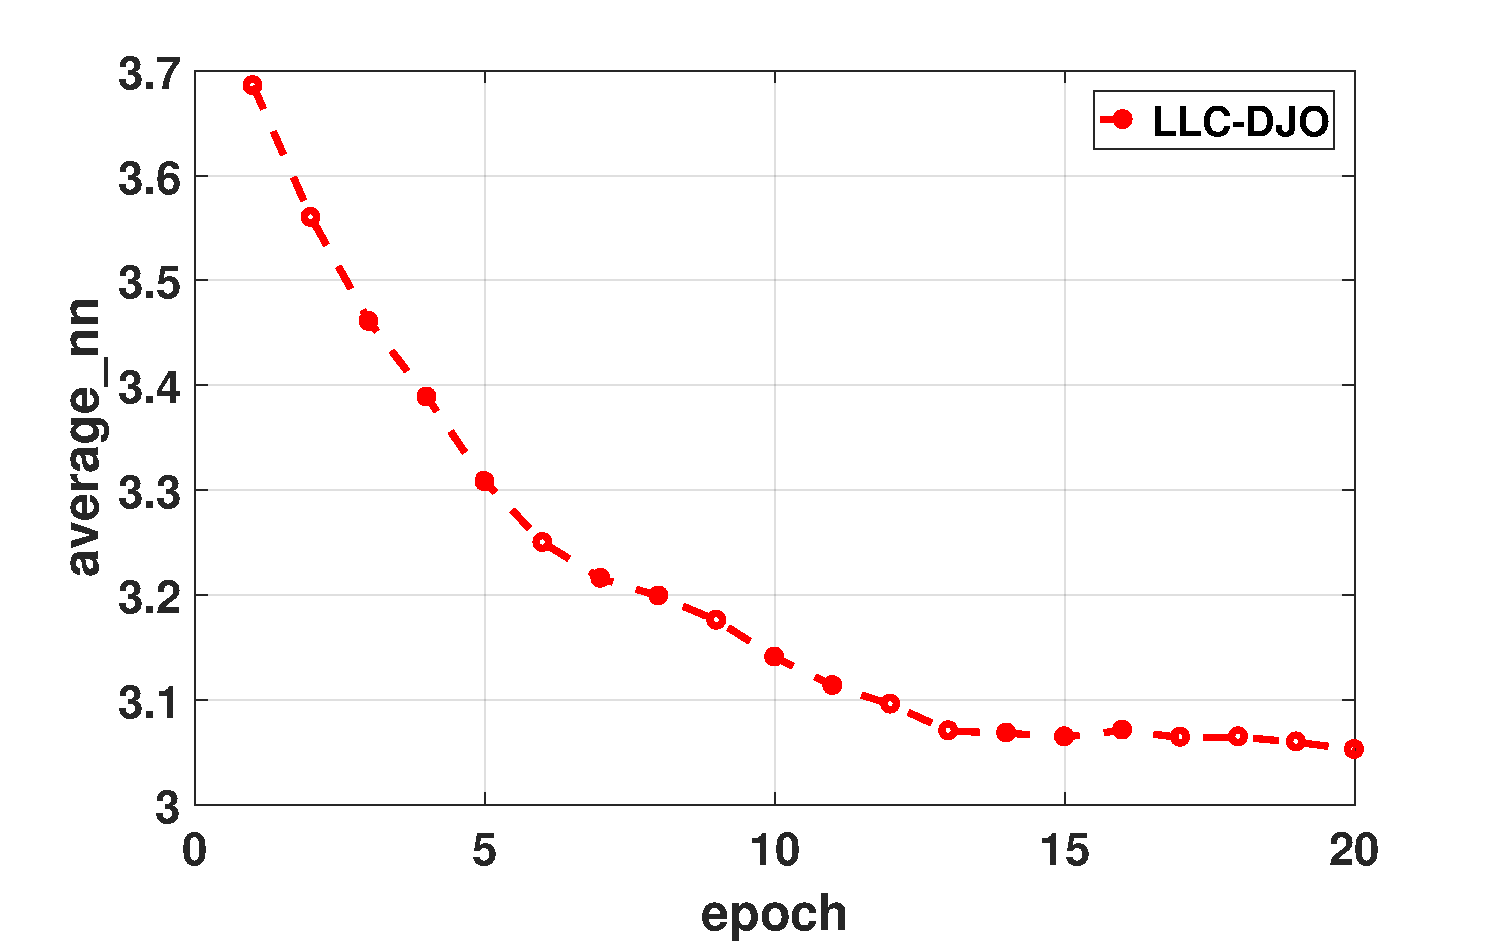
\includegraphics[width=0.5\textwidth]{ijcnn_nn.pdf}}
		\caption{Cumulative Average Number of Nearest Neighbors in learning process on Magic04 and IJCNN dataset.}
	\end{figure}

	\subsubsection{Evaluation of Parameter Sensitivity}
	For LLC-JO, Lipschitz to noise ratio $\mu$ is the key parameter. It would be interesting to explore how the algorithm may be sensitive to the setting of $\mu$. Figure 4 shows the results of parameter sensitive evaluations using different values of $\mu$. As $\mu$ grows, the number of anchor points involved in the coding phase tends to be smaller. There exists a range for $\mu$ that ensures LLC-JO outperforms LLC-SAPL, too small or too large $\mu$ will deteriorate the classification performance, which also proves that the number of anchor points involved in coding phase has a significant impact on localized soft-assignment coding scheme.
	\begin{figure}[!tbp]
		\centering
		\includegraphics[width=0.8\textwidth]{magic04_mu.pdf}
		\caption{Sensitivity of Lipschitz to noise ratio on dataset Magic04. The red line indicates the average number of nearest neighbors in test data while the blue line denotes the test hingle loss in terms of different value of $\mu$. The black line denotes the corresponding test hinge loss of LLC-SAPL baseline.}
	\end{figure}
	\section{Conclusion}
	In this paper, we propose an optimized local soft-assignment coding scheme. Different from existing localized soft-assignment coding, we formulate a joint optimization over anchor points, local coding coordinates and classifiers' variables by minimizing the distance of local approximation to the ground truth. In this novel coding scheme, the anchor points and corresponding local coding coordinates are optimized in a joint way. This design gives full consideration to that the local manifold structure may vary from data point to data point. Based on the new coding scheme, we give the algorithm for joint optimized locally linear classifier(LLC-JO). Experiment results on several benchmarks demonstrates that our algorithm achieves lower hinge loss and better predicitive accuracy than other competitive methods which employ a fixed local coding scheme.
	\begin{thebibliography}{1}
		\bibitem{1}
		Schölkopf B, Smola A J. Learning with kernels: support vector machines, regularization, optimization, and beyond[M]. MIT press, 2002.
		\bibitem{2}
		Ladicky L, Torr P. Locally linear support vector machines[C]//Proceedings of the 28th International Conference on Machine Learning (ICML-11). 2011: 985-992.
		\bibitem{3}
		Yu K, Zhang T, Gong Y. Nonlinear learning using local coordinate coding[C]//Advances in neural information processing systems. 2009: 2223-2231.
		\bibitem{4}
		Mao X, Fu Z, Wu O, et al. Optimizing Locally Linear Classifiers with Supervised Anchor Point Learning[C]//IJCAI. 2015: 3699-3706.
		\bibitem{5}
		Zhou X, Cui N, Li Z, et al. Hierarchical gaussianization for image classification[C]//Computer Vision, 2009 IEEE 12th International Conference on. IEEE, 2009: 1971-1977.
		\bibitem{6}
		Anava O, Levy K. k*-Nearest Neighbors: From Global to Local[C]//Advances in Neural Information Processing Systems. 2016: 4916-4924.
		\bibitem{7}
		Cover T, Hart P. Nearest neighbor pattern classification[J]. IEEE transactions on information theory, 1967, 13(1): 21-27.
		\bibitem{8}
		Liu L, Wang L, Liu X. In defense of soft-assignment coding[C]//Computer Vision (ICCV), 2011 IEEE International Conference on. IEEE, 2011: 2486-2493.
		\bibitem{9}
		Van Gemert J, Geusebroek J M, Veenman C, et al. Kernel codebooks for scene categorization[J]. Computer Vision–ECCV 2008, 2008: 696-709.
		\bibitem{10}
		Van Gemert J C, Veenman C J, Smeulders A W M, et al. Visual word ambiguity[J]. IEEE transactions on pattern analysis and machine intelligence, 2010, 32(7): 1271-1283.
		\bibitem{11}
		Wang J, Yang J, Yu K, et al. Locality-constrained linear coding for image classification[C]//Computer Vision and Pattern Recognition (CVPR), 2010 IEEE Conference on. IEEE, 2010: 3360-3367.
		\bibitem{12}
		Yu K, Zhang T, Gong Y. Nonlinear learning using local coordinate coding[C]//Advances in neural information processing systems. 2009: 2223-2231.
		\bibitem{13}
		Bordes A, Bottou L, Gallinari P. Sgd-qn: Careful quasi-newton stochastic gradient descent[J]. Journal of Machine Learning Research, 2009, 10(Jul): 1737-1754.
		\bibitem{14}
		Shalev-Shwartz S, Singer Y, Srebro N. Pegasos: Primal estimated sub-gradient solver for svm[C]//Proceedings of the 24th international conference on Machine learning. ACM, 2007: 807-814.
		\bibitem{15}
		Chang C C, Lin C J. LIBSVM: a library for support vector machines[J]. ACM Transactions on Intelligent Systems and Technology (TIST), 2011, 2(3): 27.
		\bibitem{16}
		Gu Q, Han J. Clustered Support Vector Machines[C]//AISTATS. 2013: 307-315.
		\bibitem{17}
		Zhang H, Berg A C, Maire M, et al. SVM-KNN: Discriminative nearest neighbor classification for visual category recognition[C]//Computer Vision and Pattern Recognition, 2006 IEEE Computer Society Conference on. IEEE, 2006, 2: 2126-2136.
		\bibitem{18}
		Wang J, Yang J, Yu K, et al. Locality-constrained linear coding for image classification[C]//Computer Vision and Pattern Recognition (CVPR), 2010 IEEE Conference on. IEEE, 2010: 3360-3367.
		\bibitem{19}
		Yang J, Yu K, Gong Y, et al. Linear spatial pyramid matching using sparse coding for image classification[C]//Computer Vision and Pattern Recognition, 2009. CVPR 2009. IEEE Conference on. IEEE, 2009: 1794-1801.
		\bibitem{20}
		Yang J, Yu K, Huang T. Supervised translation-invariant sparse coding[C]//Computer Vision and Pattern Recognition (CVPR), 2010 IEEE Conference on. IEEE, 2010: 3517-3524.
		\bibitem{21}
		Yang J, Yu K, Huang T. Efficient highly over-complete sparse coding using a mixture model[C]//European Conference on Computer Vision. Springer Berlin Heidelberg, 2010: 113-126.
	\end{thebibliography}
\end{document}